\documentclass[10pt,twocolumn,letterpaper]{article}

\usepackage{cvpr}

\usepackage{graphicx}
\usepackage{amsmath}
\usepackage{amssymb}
\usepackage{booktabs}
\usepackage[shortlabels]{enumitem}
\usepackage{tikz}
\usetikzlibrary{arrows.meta,positioning}
\usepackage[pagebackref,breaklinks,colorlinks]{hyperref}

\usepackage[capitalize]{cleveref}
\crefname{section}{Sec.}{Secs.}
\Crefname{section}{Section}{Sections}
\Crefname{table}{Table}{Tables}
\crefname{table}{Tab.}{Tabs.}

\def\cvprPaperID{*****}
\def\confName{CVPR}
\def\confYear{2026}

\begin{document}

\title{TwinWorld 2026 Challenge Final Verification Factsheet\\
Offset Sheets and Scorer-Matched Resolution for Large-Scale\\
Semantic Gaussian Splatting Reconstruction}

\author{Manish Joshi\\
Independent Researcher\\
{\tt\small manishinuae@gmail.com}
}
\maketitle

\section{Introduction}

This factsheet describes the solution submitted by team
\texttt{Manish} to the TwinWorld 2026 Challenge on large-scale 3D semantic
Gaussian Splatting reconstruction. The final submission placed 5th of 21 entries
with a final score of 1.4837, and obtained the highest geometry F-score of any
entry in the challenge (0.6386).

The pipeline is deliberately conventional in its components -- COLMAP
multi-view stereo, gsplat 3D Gaussian Splatting, and gradient-boosted trees over
local geometric descriptors -- and the contribution lies in two measurements
about how the three scored terms respond to submission-side decisions. The first
is that the semantic term, which is a nearest-neighbour label transfer within a
fixed radius and carries no precision penalty, is limited by how densely space
near the reconstructed surface is populated rather than by label quality. The
second is that the submission voxel is not a free hyperparameter but is dictated
by the evaluation protocol itself.

\section{Team details}

\begin{itemize}\itemsep2pt
\item \textbf{Team name:} \texttt{Manish}
\item \textbf{Team leader:} Manish Joshi, Independent Researcher,
      \texttt{manishinuae@gmail.com}
\item \textbf{Other team members:} none (single-participant team)
\item \textbf{Team website:} n/a
\item \textbf{Codabench user name:} \texttt{manish}
\item \textbf{Codabench ID of the final submission:} \texttt{910133}
      (Final phase, submitted 2026-08-31 15:45 UTC)
\item \textbf{Final challenge score:} 1.4837 (see \cref{tab:scores})
\item \textbf{Source code, pretrained models and checkpoints:}\\
      \url{https://huggingface.co/manishjoshiai/twinworld2026-verification}\\
      files \texttt{twinworld-code.zip} and
      \texttt{twinworld-semantic-checkpoints.tar}
\item \textbf{Complete results corresponding to the final submission:}\\
      same repository, \texttt{reconstruction/} (thirteen per-scene archives of
      the native Gaussian representation) and \texttt{submission/} (the
      submitted point clouds and renders)
\end{itemize}

The repository is private; a read-only access token scoped to it accompanies
this factsheet in the submission e-mail.

\begin{table}[t]
\centering
\begin{tabular}{@{}lr@{}}
\toprule
Metric & Value \\
\midrule
Final score      & 1.4837 \\
\midrule
PSNR             & 20.90 \\
SSIM             & 0.7432 \\
LPIPS            & 0.2996 \\
\emph{rendering} & \emph{0.6205} \\
\midrule
F-score (TUM)    & \textbf{0.6386} \\
mIoU 3D (Gold Coast) & 0.2247 \\
\bottomrule
\end{tabular}
\caption{Final-phase scores of Codabench submission 910133. The F-score is the
highest of all 21 entries in the challenge.}
\label{tab:scores}
\end{table}

\section{Method details}

\begin{figure*}[t]
\centering
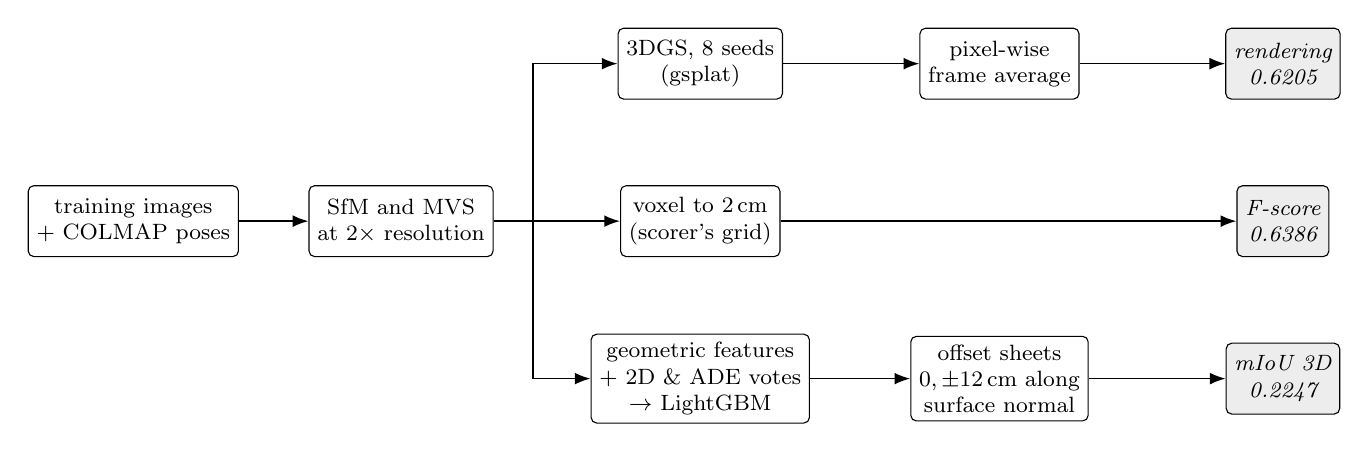
\begin{tikzpicture}[
  box/.style={draw, rounded corners=2pt, align=center, font=\footnotesize,
              minimum height=9mm, inner sep=3pt},
  res/.style={draw, rounded corners=2pt, align=center, font=\footnotesize\itshape,
              fill=black!7, minimum height=9mm, inner sep=3pt},
  ar/.style={-{Latex[length=2mm]}, semithick}]

\node[box] (in) at (0,0) {training images\\+ COLMAP poses};
\node[box] (mvs) at (3.4,0) {SfM and MVS\\at $2\times$ resolution};

\node[box] (gs)   at (7.2,2.0) {3DGS, 8 seeds\\(gsplat)};
\node[box] (avg)  at (11.0,2.0) {pixel-wise\\frame average};
\node[res] (rend) at (14.6,2.0) {rendering\\0.6205};

\node[box] (vox)  at (7.2,0) {voxel to 2\,cm\\(scorer's grid)};
\node[res] (tum)  at (14.6,0) {F-score\\0.6386};

\node[box] (cls)  at (7.2,-2.0) {geometric features\\$+$ 2D \& ADE votes\\$\rightarrow$ LightGBM};
\node[box] (sh)   at (11.0,-2.0) {offset sheets\\$0,\pm12$\,cm along\\surface normal};
\node[res] (miou) at (14.6,-2.0) {mIoU 3D\\0.2247};

\draw[ar] (in) -- (mvs);
\draw[ar] (mvs.east) -- ++(0.5,0) |- (gs.west);
\draw[ar] (mvs.east) -- (vox.west);
\draw[ar] (mvs.east) -- ++(0.5,0) |- (cls.west);
\draw[ar] (gs) -- (avg);
\draw[ar] (avg) -- (rend);
\draw[ar] (vox) -- (tum);
\draw[ar] (cls) -- (sh);
\draw[ar] (sh) -- (miou);
\end{tikzpicture}
\caption{Pipeline. One shared reconstruction front end feeds three independent
branches, one per scored term. The two contributions are on the right-hand side
of the lower branches: submitting TUM at the scorer's own 2\,cm grid rather than
a coarser one, and thickening the labelled Gold Coast cloud perpendicular to its
surface so that ground truth displaced from our reconstruction still falls
within the 10\,cm match radius. Values shown are the final-phase scores of
submission 910133.}
\label{fig:pipeline}
\end{figure*}

\subsection{Overall pipeline}

\Cref{fig:pipeline} summarises the pipeline.

The pipeline has three branches, one per scored term, sharing a common
structure-from-motion and multi-view stereo front end.

\begin{enumerate}[1.]\itemsep2pt
\item \textbf{Front end.} The provided COLMAP poses are used as given. Training
images are upsampled $2\times$ with Lanczos resampling before undistortion, with
intrinsics scaled to match, and dense reconstruction is run with a permissive
photometric-consistency setting. Per-scene depth maps are fused into a point
cloud, and a union of fusion passes is retained per scene.

\item \textbf{Rendering branch.} 3D Gaussian Splatting is optimised per scene
with gsplat and the test poses are rendered. Eight independently seeded models
are trained per scene and their rendered frames are averaged pixel-wise.

\item \textbf{Geometry branch (TUM).} The fused MVS cloud is voxel-downsampled
to 2\,cm and submitted directly.

\item \textbf{Semantic branch (Gold Coast).} Per-point features are classified
into the five challenge classes, the labelled cloud is thickened perpendicular to
its own surface, and the result is submitted with per-point labels.
\end{enumerate}

\subsection{Rendering}

Gaussian models are optimised with gsplat using spherical harmonics of degree 3,
the default densification strategy, antialiased rasterisation, and a
D-SSIM weight of $0.2$. Two per-dataset settings were selected on the
development scenes: Gold Coast uses the sparse SfM points as initialisation and
7000 iterations, while TUM initialises from the dense MVS cloud and uses 3000
iterations. Densification stops at 72\% of the schedule.

Repeating an identical configuration on a Gold Coast development scene produced
a rendering score between 0.5103 and 0.5386 across three runs -- a standard
deviation of 0.014, against 0.0018 on TUM. The held-out Gold Coast views
extrapolate 16--18\,m from the nearest training camera, so small differences in
densification move the rendered image substantially. Averaging eight
independently seeded runs is therefore variance reduction, and it improves all
three rendering metrics simultaneously, including LPIPS, which frame averaging
normally harms: the floaters each run invents independently cancel, while the
geometry the runs agree on does not. Nothing about the held-out image is used to
combine the runs.

\subsection{Geometry and the submission voxel}

Image resolution, not MVS parameter tuning, was the binding constraint on TUM
geometry. The ground sampling distance is about 3.4\,cm/px at 36\,m altitude
while the ground truth is a 2\,cm scan. Upsampling the input images $2\times$
improved mean F from 0.4758 to 0.5336 on a development scene, with F@5 improving
by 47\%; by comparison, an entire sweep over MVS filtering settings moved the
mean by 0.002. A $4\times$ variant was also reconstructed and measured, and it
\emph{lost} to the retained fusion union (0.5539 against 0.5905), so it was not
adopted.

The submission voxel proved equally consequential and is a property of the
evaluation protocol rather than a tunable. The scorer voxel-downsamples both the
submitted and reference clouds to 2\,cm before matching, so a submission coarser
than 2\,cm discards resolution the scorer would have used, while a submission
finer than 2\,cm contributes points that are immediately merged. Measured on a
development scene:

\begin{table}[h]
\centering
\begin{tabular}{@{}lrr@{}}
\toprule
Submission voxel & Points & Mean F \\
\midrule
4\,cm & 5.17\,M & 0.5698 \\
\textbf{2\,cm} & 8.37\,M & \textbf{0.5905} \\
\bottomrule
\end{tabular}
\caption{TUM geometry against the submission voxel, development scene.}
\end{table}

\subsection{Semantic labelling}

Labels are produced by a LightGBM classifier over a concatenation of three
feature groups, fitted on the two labelled Gold Coast scenes and applied to the
withheld ones.

\textbf{Geometric features.} Local structure-tensor descriptors -- linearity,
planarity, sphericity, verticality, log local extent, and signed offset from the
locally fitted plane -- computed at several neighbourhood sizes, together with
height above a local terrain model and signed height relative to the local roof
plane. Neighbourhoods are $k$-nearest rather than radius-based so the descriptor
is scale-adaptive.

\textbf{Learned 2D votes.} The provided 3D semantic ground truth is projected
into the training views to synthesise 2D masks, which requires no additional
annotation. A SegFormer \texttt{mit-b0} backbone is fine-tuned on those masks and
its per-view predictions are lifted back to 3D by projecting every point into
every view and accumulating a vote histogram. A depth buffer over our own cloud
suppresses votes collected by occluded points. This addresses a failure that
geometry cannot: a window is coplanar with its wall, so plane offset,
verticality and curvature are identical for both, while in image space windows
are 18\% of labelled pixels.

\textbf{Zero-shot votes.} A SegFormer-B2 model fine-tuned on ADE20K is applied
without adaptation and its 150 classes are mapped into eight super-groups
(building, window, road/ground, vegetation, vehicle, sky, object, water). These
votes are projected with the same occlusion-aware procedure. This recovers
label-to-class conversion in regions where 23 training images per scene are
insufficient.

Predictions are made on a thinned cloud and propagated to the full submission
cloud by $k{=}5$ nearest-neighbour majority vote.

\subsection{Offset sheets}

The semantic metric assigns each ground-truth point the label of the nearest
submitted point within 10\,cm and counts unmatched points as errors. It applies
no penalty for submitted points that are wrong or superfluous. Our reconstructed
surface sits a median 13.8\,cm from the ground truth, so a majority of the
ground truth was unmatchable irrespective of label quality, and the measured
coverage as a function of match radius (0.42 at 10\,cm, 0.71 at 20\,cm, 0.90 at
50\,cm) shows the mass is present but displaced.

Densifying \emph{along} the surface cannot address this, because additional
points land on the same displaced surface. The submitted cloud is therefore
thickened \emph{perpendicular} to it: each point emits copies at $\pm12$\,cm
along its local surface normal, carrying its parent's label. Normals are fitted
by local PCA on the clean 10\,cm surface cloud and oriented towards the camera
rig, then inherited by the packed cloud.

Configurations were ranked by an analytic estimator. Because the metric depends
only on which point wins the nearest-neighbour race, the distance from a
ground-truth point $g$ to the sheet of a parent $p$ with unit normal $n$ at
offset $o$ is
\[
\|d - o\,n\|^2 = \|d\|^2 - 2\,o\,(d\!\cdot\!n) + o^2, \qquad d = g - p ,
\]
so a single $k$-nearest-neighbour query of the ground truth against the parents
prices every offset configuration in closed form without materialising any
sheet. The estimator reproduced the reference scorer exactly on both labelled
scenes.

Three findings determined the shipped configuration. The gain must be bought
with additional points and cannot be reallocated: every budget-matched variant,
in which parents were coarsened to pay for the sheets, was neutral or worse, and
coarsening past roughly 15\,cm breaks lateral coverage because the worst-case
in-plane gap then exceeds the 10\,cm match radius. Reach matters more than sheet
count, up to a saturation near $\pm18$\,cm. And the effect reverses at long
range: a stack reaching $\pm54$\,cm achieved the highest coverage measured
anywhere in our experiments and the \emph{lowest} mIoU of any sheeted
configuration, because a copy displaced half a metre carries a label sampled too
far away to be informative and, being nearer to the ground-truth point than the
honest surface behind it, displaces a label that would have been correct.

\subsection{External data and models}

\textbf{Do you use extra data besides the competition data provided?}
\textbf{No.} All reconstruction, all classifier training and all Gaussian
optimisation used only the challenge-provided images, poses and labels. No
additional imagery, point clouds or annotations of any kind were introduced.
The 2D masks used to supervise the segmenter were not annotated: they are
synthesised by projecting the challenge's own 3D semantic ground truth into the
training views.

Two publicly available pretrained \emph{models} were used, and are disclosed
here in full:

\begin{itemize}\itemsep2pt
\item \texttt{nvidia/mit-b0} -- SegFormer~\cite{xie2021segformer} backbone with
ImageNet pretraining, fine-tuned on 2D masks synthesised by projecting the
challenge's own 3D labels. No external segmentation annotation was used.
\item \texttt{nvidia/segformer-b2-finetuned-ade-512-512} -- SegFormer fine-tuned
on ADE20K~\cite{zhou2017ade20k}, applied zero-shot with its output classes
mapped to eight super-groups.
\end{itemize}

Third-party software: COLMAP~\cite{schoenberger2016sfm} for SfM and MVS,
gsplat~\cite{ye2024gsplat} for Gaussian Splatting, LightGBM~\cite{ke2017lightgbm}
for classification.

\subsection{Novelty and prior publication}

None of this work has been previously published, and no part of it is under
review elsewhere. It was developed entirely within the challenge period.

The components are all established: COLMAP for structure-from-motion and
multi-view stereo, gsplat for Gaussian Splatting, SegFormer for 2D segmentation,
and gradient-boosted trees for point classification. We claim no novelty for any
of them, and we would not describe the solution as a new method.

What we would put forward as contributions are two measurements about the
evaluation protocol, both of which we believe are of interest beyond our own
submission. The first is that the semantic metric -- a nearest-neighbour label
transfer within a fixed radius, with no precision penalty -- is bounded by how
densely space near the reconstructed surface is populated rather than by label
quality, and that thickening the cloud perpendicular to its surface exploits
this, but saturates and then reverses once the displacement exceeds roughly a
quarter of a metre because coverage and label conversion are not independent.
The second is that the submission voxel is dictated by the scorer's own
downsampling grid rather than being a free hyperparameter, which we established
only on the final day of the challenge and which was worth more per unit of
effort than anything else we attempted.

The offset-sheet operation itself is, as far as we are aware, not standard
practice; whether it should be is a separate question, and \cref{sec:other}
argues that a symmetric metric would remove the incentive for it.

\subsection{Complexity and runtime}

Per Gold Coast scene, a single Gaussian model converges to roughly 0.9\,M
Gaussians in about 140\,s on one NVIDIA A100-80GB; the eight-member ensemble
costs about 19 minutes per scene. MVS at $2\times$ resolution is the dominant
cost at roughly 700--1700\,s per scene. The semantic classifier is a
200-estimator LightGBM model and trains in minutes on CPU. Sheet materialisation
and packaging are CPU-only and take under 10 minutes for the whole submission.
Peak GPU memory during Gaussian optimisation is under 40\,GB.

\section{Ensemble and Fusion Strategies}

Two fusion strategies are used, at different stages.

\textbf{Rendering ensemble.} Eight independently seeded Gaussian models per
scene, averaged pixel-wise in image space. This was adopted because per-run
variance on Gold Coast is an order of magnitude larger than on TUM, and
averaging beats not only the mean single run but the best single run while
improving PSNR, SSIM and LPIPS simultaneously. An MCMC densification variant was
measured as an alternative and rejected: it improved PSNR markedly (21.99
against 19.94) but degraded LPIPS enough (0.457 against 0.418) to lose overall,
0.5650 against 0.5759.

\textbf{Semantic feature fusion.} The classifier consumes geometric descriptors,
supervised 2D votes and zero-shot ADE20K votes as a single concatenated feature
vector rather than combining three separate predictions. Each group contributes
where the others fail: geometry cannot express a window, the supervised
segmenter is limited by 23 images per scene, and the zero-shot model has no
notion of the challenge's class definitions but is reliable on building,
vegetation and ground. Adding the zero-shot group to the previously adopted
stack improved leave-one-scene-out mIoU by 0.0047.

Every candidate throughout the challenge was admitted through a fixed gate:
both leave-one-scene-out folds had to improve over their own baselines and the
pooled score had to beat the incumbent. Roughly 90 configurations were evaluated
and the large majority were rejected under this rule, including nine consecutive
attempts to improve semantics by increasing model capacity or training schedule.

\section{Other Details}
\label{sec:other}

\textbf{Impressions.} The challenge is well designed in that the three scored
terms genuinely pull in different directions, and the Gold Coast semantic task
is a real research problem rather than a tuning exercise: two labelled scenes
are not enough supervision for the withheld ones, and our nine rejected capacity
experiments reflect that rather than any shortage of effort.

\textbf{Difficulties.} The dominant difficulty was that the submission envelope
was never documented. An early submission failed at 108.6\,M points and we
inferred a size limit from it, then spent ten days optimising under a point
budget that did not exist -- the Final phase in fact specifies no size limit at
all, only a 6000\,s execution-time cap, and the figure we had inferred was
almost certainly the Development phase's tighter time limit. Recognising this on
the final day and restoring TUM to the scorer's own 2\,cm grid was worth 0.011 of
final score for one measurement, more per unit of effort than anything else
attempted in the last week of the challenge.

\textbf{Comments on the evaluation.} The semantic metric's asymmetry -- a
nearest-neighbour transfer with no precision penalty -- rewards filling space
near the surface, which is a submission-side strategy rather than a
reconstruction improvement. Our own results illustrate both the exploit and its
limit: sheets are worth roughly $+0.042$ of final score, but the effect saturates
and then reverses, because coverage and label conversion are not independent. A
symmetric metric, or a cap on submitted points relative to the reference cloud,
would remove the incentive without weakening the task. Publishing the size and
runtime limits explicitly would also help; we are unlikely to have been the only
team to misread a failed submission as a size limit.

\textbf{Suggestions.} A semantic sub-track evaluated at several match radii would
separate reconstruction accuracy from space filling, and would have made visible
much earlier that the leading teams' advantage was that their surfaces fall
inside the 10\,cm radius to begin with, rather than that they submit more points.

{\small
\bibliographystyle{ieeenat_fullname}
\bibliography{egbib}
}

\end{document}
